
\documentclass[main.tex]{subfiles}

\begin{document}

\chapter{Cohesive zone, softening, energy dissipation}
\label{LEC:CohesiveCrackModel}

The notion of energy dissipation, localization and fracture process zone is useful for two purposes:
\begin{itemize}
    \item regularization of the finite element computation
    \item size effect on the structural response
\end{itemize}
In the former case, energy dissipation rate is used as a material parameter 
to remove mesh dependency from the numerical calculation. 
The latter case represents an important phenomenon that has to be accounted for in the safety assessment
of structures. Let us demonstrate the effect of strain softening on the 
results of the finite element calculation.

\section{Sensitivity of strain-softening models with respect to size of the localization zone}

\begin{figure}[ht]
	\centering
  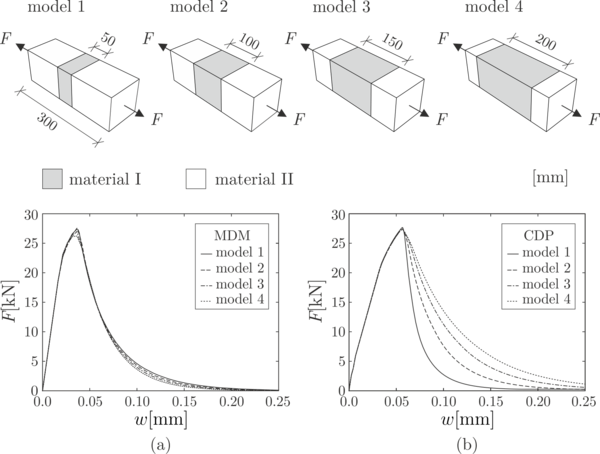
\includegraphics[width=0.8\textwidth]{fig/Lecture07/mesh_sensitivity.png}
	\caption{Finite-element computation of with a softening zone}
	\label{FIGDrawingEnergyPullout}
\end{figure}

The example in Fig.~\ref{FIGDrawingEnergyPullout} shows the calculated response of a tensile test using finite element method with three different sizes of the middle section exhibiting a lower strength than the outer regions.

The structural response calculated with two different models is shown in terms of the tensile force  versus the control displacement. The bottom-right diagram shows the different curves obtained using the damage-plasticity model in Abaqus.

The sensitivity of the softening branch with respect to the size of the softening volume can be explained using elementary analysis of a tensile test with a cohesive zone. The basis for this analysis can be provided using the cohesive crack model.
\begin{align}
\sigma = E \varepsilon_\mathrm{el}
\end{align}
and the softening law
\begin{align}
\sigma = f(w)
\end{align}
defining the decay of stress  with an increasing crack opening. In the considered case of the tensile test, the stress level in a series of two springs representing the bulk material and the cohesive crack is constant so that we exploit the equilibrium condition to relate the elastic strain to the softening function as
\begin{align}
\sigma = \mathrm{constant.} \implies f(w) = E \varepsilon_\mathrm{el}
\implies \varepsilon_\mathrm{el} = \frac{f(w)}{E}
\end{align}
The control displacement $u$ is given as a sum of the elastic elongation $\varepsilon_{\mathrm{el}} L$ and the crack opening  $w$
\begin{align}
u = \varepsilon_{\mathrm{el}} L  + w = L \frac{f(w)}{E} + w
\end{align}
Evidently, the load-elongation curve in tensile test under monotonic extension is completely determined by $L$, $E$  and $f(w)$.  Finally, we obtain the effective strain of the tensile test in the softening regime using the kinematic condition and substituting the terms above as
\begin{align}
\varepsilon(w) = \frac{u}{L} = \varepsilon_\mathrm{el}  + \frac{w}{L}
= \frac{1}{E} \sigma + \frac{w}{L}
= \frac{1}{E} f(w) + \frac{w}{L}
\end{align}
so that we can calculate the global strain for monotonically increasing crack opening. The corresponding value of stress is given by the softening law
\begin{align}
\sigma(w) = f(w)
\end{align}
For $L \rightarrow \infty$ we get $\frac{w}{L} \rightarrow 0$ then 
$\varepsilon(w) = \frac{1}{E} \sigma(w)$
this means that for arbitrary value of crack opening, the quasi-static unloading  is only possible by following the linear-elastic branch back to the origin. strain and stress remains linear even upon unloading.

\section{Softening function accounting for fracture energy}

To explain the role of energy dissipation in the numerical calculation let us introduce
a softening containing the fracture energy as its parameter. The shape of the softening function
is assumed in exponential form scaled by two parameters $c_1$ and $c_2$
\begin{align}
\sigma = c_1 \exp( -c_2 w ).
\end{align}
The parameter $c_1$ can be set equal to the tensile strength $f_\mathrm{t}$ 
accounting for the fact that softening starts 
at the level of the material strength 
\begin{align}
\sigma(0) = f_t \implies  c_1 = f_t.
\end{align}
The parameter $c_2$ is obtained by requiring that the energy dissipated 
by a unit surface area of a crack equals 
the fracture energy
\begin{align}
G_\mathrm{F} & = \int_0^\infty \sigma(w) \; \mathrm{d}w
=
\int_0^\infty c_1 \exp( -c_2 w ) \; \mathrm{d} w 
= 
f_t \left[  -\frac{1}{c_2} \exp(-c_2 w) \right]_0^\infty \nonumber \\
& = 
\frac{f_t}{c_2}
\implies
c_2 = \frac{f_t}{G_\mathrm{F}}.
\end{align}
With these two parameters the softening function has the form
\begin{align}
\label{eq:fracture_based_cohesive_law}
\sigma = f(w) = f_t \exp\left( - \frac{f_t}{G_\mathrm{F}} w \right).
\end{align}
This kind of definition is particularly suitable for explaining the 
relation between the softening law of a crack surface accounting for the
dissipated fracture energy and the energy dissipation due to 
localized damage in the finite element computations.  

\section{Energy dissipation for strain softening}
To quantify the energy dissipation at a particular value of crack opening  we need to evaluate the energy supply and the energy still stored in the specimen during the softening process:

\paragraph{Work energy supply} To evaluate the total energy supplied into the tensile specimen we can consider the influx of energy separately for the elastic bulk material and for the softening cross section where the crack develops
\begin{align}
W = W_\mathrm{el} + W_\mathrm{cr}
\end{align}
The elongation of the elastic part of the specimen is given as
\begin{align}
u_\mathrm{el} = \varepsilon_\mathrm{el} L = \frac{\sigma}{E} L
\end{align}
with the work supply equal to that given previously in Eq.~(\ref{eq:elastic_energy_supply})
\begin{align}
W_\mathrm{el} = \frac{1}{2} A \sigma u_\mathrm{el}
=
\frac{1}{2E} A L \sigma^2
=
\frac{1}{2E} A L f^2(w)
\end{align}
The work within the softening cross section is performed on the crack-opening displacement
\begin{align}
W_\mathrm{cr}
= A \int \sigma \; \mathrm{d} w
= A \int f(w) \; \mathrm{d} w
\end{align}
So that the sum reads
\begin{align}
W = \frac{1}{2E} A L f^2(w) + A \int f(w) \; \mathrm{d} w.
\end{align}

\paragraph{Stored energy:} The specimen can be regarded as a series of springs: one for the elastic bulk material and one for the cohesive crack. The volume integral over the two different parts of the specimen can be again split into the elastic unloading and into the softening parts.
\begin{align}
\mathcal{U} = 
\frac{1}{2} 
\int_\Omega \sigma \varepsilon(x) \; \mathrm{d}\Omega
=
\frac{1}{2} 
A
\int_{\Omega_\mathrm{el}}
\sigma \varepsilon_\mathrm{el}
\; \mathrm{d} x
+
\frac{1}{2} 
A
\sigma w 
=
\frac{1}{2} 
A 
\left(
L
\sigma \varepsilon_\mathrm{el}
+
\sigma w 
\right).
\end{align}
Recalling that during the unloading branch we can set
\begin{align}
\varepsilon = \frac{1}{E} f(w).
\end{align}
we obtain
\begin{align}
\mathcal{U} = 
\frac{1}{2} A 
\left(  
\frac{L }{E} 
  f^2(w) 
+ f(w) w 
\right)
= 
\frac{1}{2E} A  L
  f^2(w) 
+ 
\frac{1}{2} A 
 f(w) w.
\end{align}
The total energy released at the crack opening 
\begin{align}
G = W - \mathcal{U}
\end{align}
thus reads
\begin{align}
G &= \frac{1}{2E} AL\left( f^2(w) - f^2(w) \right) +
 A\left(  \int f(w) \mathrm{d}w -  \frac{1}{2} f(w) w  \right)
 \\ \nonumber
&=
 A\left(  \int f(w) \mathrm{d}w -  \frac{1}{2} f(w) w  \right).
\end{align}
For $w \rightarrow \infty$ we realize that $f(w) \rightarrow 0$  so that the second term will vanish for large crack opening. As a consequence, we can conclude that the total value of fracture energy $G_\mathrm{F}$ required to make the crack stress-free is
\begin{align}
G = 
 A  \int f(w) \mathrm{d}w  
=
 A   G_\mathrm{F}.
\end{align}
This is the expected result rephrasing that  $G_\mathrm{F}$ represents the energy dissipated through a unit area of a stress-free crack face.

\paragraph{Remark:} In the above evaluation of fracture energy, the work supply into the elastic part of the specimen and the amount of stored energy cancel. Therefore, evaluation of the dissipated energy can be limited to the volume of the softening spring. Thus, the dissipated energy owing to cracking can be evaluated locally, ignoring the elastic part of the specimen. This observation is useful for further elaboration on the size of the localization zone characteristic for the particular concrete mixtures.

\begin{bmcsex}{Tensile behavior of a specimen with a softening zone}{e61_length_dependence}
Consider a chain of springs with softening behavior. The spring chain can be regarded as the simplest possible discretization of a tensile specimen of a length $L$. Test the force-displacement response for varying length of the specimen using the script \href{https://wiki.imb.rwth-aachen.de/do/view/IMB/Teaching/TeachExampleObj0017}{length dependence}.

\paragraph{Questions}
\begin{itemize}
\item
How does the tensile test response change with varying specimen length?
\item
How dost the tensile test response change with the change of the softening zone length $L_\mathrm{s}$.
\item
How does the tensile test response change if the fracture energy is very large/very low? 
\item
Is snap-back a physical property? 
\item
Can the snap-back be measured experimentally?
\end{itemize}

\end{bmcsex}

\section{Correspondence between softening and damage functions}

To embed the concept of the controlled energy dissipation within a finite element calculation we establish a link between the softening law and the damage function. Indeed, by deriving the damage function from the softening law, we obtain an implicitly regularized strain-softening model demonstrating the approach used in the most commercial codes.

The behavior of a material point can be decomposed into linear-elastic and inelastic, i.e. general strain-softening material behavior as follows
\begin{align}
\sigma(\varepsilon) = \left\{ 
\begin{array}{ll}
E \varepsilon  &   \varepsilon \le \varepsilon_0 \\
\phi(\varepsilon - \varepsilon_0) 
 &  \varepsilon > \varepsilon_0
\end{array}
\right.
\end{align}
In order to show the correspondence with the previously used cohesive crack law 
\begin{align}
\label{EQ:softening_exp}
\sigma = f(w) = f_t \exp\left( - \frac{f_t}{G_\mathrm{F}}w \right)
\end{align}
let us now incorporate the the strain-softening function  into the framework of a damage model within a finite element computation. Using the softening function governed by the fracture energy we introduce the finite length of the softening zone $L_\mathrm{s}$ as a parameter. Then we can set 
\begin{align}
\label{EQ:strain_based_softening_exp}
\phi(\varepsilon - \varepsilon_0) = f( w=(\varepsilon-\varepsilon_0) L_\mathrm{s})
=
f_t \exp\left( - \frac{f_t}{G_\mathrm{F}} (\varepsilon-\varepsilon_0) L_\mathrm{s} \right)
\end{align}

The decomposed representation of the material behavior in terms of the softening law should be equally well reproducible using a damage model describing the strain-softening as a material deterioration, which has been discussed in Chapter %\ref{LEC:CohesiveCrackModel} 
in the context of approaches to interface modeling. as
\begin{align}
\sigma(\varepsilon) = (1 - \omega) E \varepsilon
\end{align}
where $\omega$ is a monotonic damage function with values within the range (0,1). 
The damage function can be related to the softening function introduced above in the following way. For $\varepsilon \le \varepsilon_0$ we obtain $\omega = 0$ and for the softening regime $\varepsilon > \varepsilon_0 $ the damage function reads
\begin{align}
\omega(\varepsilon) = \left\{ 
\begin{array}{ll}
0  &   \varepsilon \le \varepsilon_0 \\
1 - \displaystyle{\frac{ \phi(\varepsilon - \varepsilon_0) }{E \varepsilon }}
 &   \varepsilon > \varepsilon_0
\end{array}
\right.
\end{align}
Substituting from (\ref{EQ:strain_based_softening_exp}) we obtain a strain-based damage function with fracture energy $G_\mathrm{F}$ and tensile strength $f_t$ as parameters 
\begin{align}
\label{eq:damge_fn_fracture_base_exp}
\omega(\varepsilon) = \left\{ 
\begin{array}{ll}
0  &   \varepsilon \le \varepsilon_0 \\
1 - \displaystyle{\frac{ 1 }{E \varepsilon }}
f_t \exp\left( - \frac{f_t}{G_\mathrm{F}} \left(\varepsilon - \varepsilon_0\right) L_\mathrm{s} \right)
 &   \varepsilon > \varepsilon_0
\end{array}
\right.
\end{align}
Deriving a material law with physically meaningful parameters is certainly aesthetically pleasing. However it does not provide us any guarantee that the model will be able to capture the real behavior. Notice that the choice of the exponential function (\ref{eq:fracture_based_cohesive_law}) was rather intuitive. Other choices, e.g. bi-linear might be taken as well.
Nevertheless, the fact that the parameters of damage function have a clear physical interpretation can be exploited during the model calibration as we will discuss in Chapter~\ref{LEC:CrackPropagation}. 

\begin{bmcsex}{Transformation of a softening function to damage function}{ex71_softening_to_damage} 
The derivation is provided in an interactive form in the 
\href{http://localhost:8888/tree/Examples/7_2_Crack_softening_law_and_damage_function.ipynb}{jupyter notebook}.

\paragraph{Questions}
\begin{itemize}
\item What is the unit of fracture energy?
\item What is the unit of energy release rate?
\item 
How does the fracture energy influence 
the relation between the stress and crack opening?
\item
How does the equivalent parameter $L_\mathrm{s}$ in the 
damage function influence the stress strain response?
\end{itemize}
\end{bmcsex}


\end{document}